% ==============================================================================
%  Consistency Is Not Correctness: single-answer vs multi-sample black-box UQ
%  ACL-format paper. Requires the official ACL style files in this directory:
%    acl.sty, acl_natbib.bst   (from https://github.com/acl-org/acl-style-files)
%  Compile:  pdflatex main ; bibtex main ; pdflatex main ; pdflatex main
% ==============================================================================
\documentclass[11pt]{article}

\usepackage[review]{acl}
\usepackage{latexsym}
\usepackage[T1]{fontenc}
\usepackage[utf8]{inputenc}
\usepackage{microtype}
\usepackage{booktabs}
\usepackage{amsmath}
\usepackage{amssymb}
\usepackage{multirow}
\usepackage{graphicx}
\usepackage{xcolor}
\usepackage{url}
\usepackage{enumitem}
\usepackage{pgfplots}
\pgfplotsset{compat=1.17}
\usepgfplotslibrary{groupplots}

\newcommand{\best}[1]{\textbf{#1}}
\newcommand{\grey}[1]{\textcolor{gray}{#1}}
\newcommand{\nverb}{$n_1$}     % verbalized floor
\newcommand{\nphi}{$n_3$}      % deterministic phi CoI
\newcommand{\nyn}{$n_6$}       % decision-framed verify
\newcommand{\nsc}{$n_7$}       % self-consistency verify

\title{Consistency Is Not Correctness: When Single-Answer Uncertainty \\
Beats Multi-Sample Estimation in Black-Box LLMs}

% author block omitted: [review] mode emits "Anonymous ACL submission".
% CAMERA-READY: restore \author{...} here.
\begin{document}
\maketitle

\begin{abstract}
The dominant black-box uncertainty estimators resample a language model and measure how much
its answers disagree. This works only if the model's errors are \emph{inconsistent}. We ask where
that assumption holds, comparing \emph{single-answer} estimators---which score one fixed answer,
paying no extra generations---against \emph{multi-sample} consistency and graph-spectral methods
across six targets (8B to 70B open, plus GPT-4o and Claude-Haiku) and twelve datasets. The answer
is sharply structured by data type. On \textbf{adversarial} content the single-answer family wins
\textbf{4 of 4} cells by a median $+0.169$ AUROC, and on \textbf{multiple-choice health} \textbf{5
of 6} by $+0.088$: TruthfulQA is the extreme case, where every multi-sample baseline sits at or
below chance on Llama-3.3-70B ($0.49$--$0.54$) while a single verbalized call reaches $0.782$.
Imitative falsehoods and confident wrong options are produced \emph{consistently}, so dispersion
carries no signal. Where errors are inconsistent---general-knowledge
short-form ($1/8$) and long-form ($0/2$)---multi-sample methods win, though they need up to ten
extra generations of the full answer to do it. Within the single-answer family we ablate seven
scoring rules and find no universal winner; the useful contribution is the \emph{selection rule},
not a new estimator. We report bootstrap intervals and exclude class-imbalanced cells. Finally, scoring the closed
targets twice two days apart---identical items, labels and greedy decoding---moved $12$ of $32$
comparisons by over $0.10$ AUROC, so closed-model numbers are not reproducible without a pinned
provider snapshot. Harness and per-item scores released.
\end{abstract}

\section{Introduction}
Deployed systems increasingly consume answers from language models they cannot inspect: no
logits, no hidden states, no weights, only text. The dominant uncertainty estimators for this
setting are \emph{multi-sample}: resample the model several times and measure how much the
answers disagree, via semantic-entropy clustering~\citep{kuhn2023semantic,farquhar2024detecting}
or graph-spectral scores over the sample set~\citep{lin2024generating}. They are strong, widely
used, and rest on an assumption that is rarely stated: that when a model is wrong, it is
\emph{unsure}---that its errors show up as disagreement among resamples.

That assumption fails in an important class of cases. A model reproducing a common human
misconception, or confidently selecting the wrong multiple-choice option, will produce the
\emph{same} wrong answer every time. Dispersion is then zero and the estimator is blind, however
many samples it draws. Where this happens, the alternative is a \emph{single-answer} estimator:
one that scores the one answer already produced---by asking the model to rate it
\citep{tian2023just,kadavath2022language}, by decomposing it into claims and scoring each, or by
re-verifying each claim discriminatively---and therefore pays no additional generations at all.

This paper maps where each family works. We evaluate both across six targets (8B to 70B open,
plus GPT-4o and Claude-Haiku) and twelve datasets spanning short- and long-form, multiple-choice,
adversarial, math and multi-hop content, every method scoring the same cached generations.\footnote{Harness, per-item scores and analysis scripts:
\url{[repository URL withheld for anonymous review]}} Within the single-answer family we also
ablate seven scoring rules, from a single global self-rating to $K$-vote discriminative
verification, to see which part of the machinery carries the signal.

We compare the two families across a $6\times12$ grid and report four findings
(\S\ref{sec:results}).
\begin{enumerate}[leftmargin=1.4em,itemsep=1pt,topsep=2pt]
\item \textbf{Which family wins is determined by the data, not the model.} Over $29$
non-degenerate cells where both families were run, single-answer estimators win $12$. But the
split is not random: they take $4/4$ adversarial cells and $5/6$ multiple-choice health cells,
and lose $1/8$ general short-form and $0/2$ general long-form.
\item \textbf{Sampling fails exactly when errors are consistent.} Multi-sample methods estimate
uncertainty from disagreement among resamples, so they are blind to errors a model makes
\emph{reliably}. TruthfulQA is the clean case: its imitative falsehoods are generated
consistently, and on Llama-3.3-70B every multi-sample baseline lands at $0.49$--$0.54$ while
plain verbalized confidence reaches $0.782$. Multiple-choice health behaves the same way---a
model that confidently picks the wrong option picks it every time.
\item \textbf{Where sampling works, it is worth its cost---but the cost is real.} On
general-knowledge short-form the multi-sample methods win $7$ of $8$ cells, and on long-form both,
but only at $N{=}10$: ten additional generations of a $180$-word answer against the single
generation the answer already cost. At $N{=}5$ the two families are level on long-form.
\item \textbf{Closed-target results are not reproducible across provider snapshots.} Scoring
GPT-4o and Claude-Haiku twice through the same gateway two days apart---same cached answers,
labels and items, greedy decoding, zero failed calls---moved $12$ of $32$ comparisons by more
than $0.10$ AUROC and removed both cells behind an inversion finding we had previously drawn.
We report the second run, release both, and recommend that black-box evaluations record the
resolved snapshot id per cell (\S\ref{sec:inversion}).
\item \textbf{Within the single-answer family, no scoring rule dominates.} We ablate seven
(\S\ref{sec:method}): a global self-rating, per-claim self-ratings, a deterministic aggregation
over self-rated risk, and discriminative yes/no verification asked once or $K$ times. Each is
best somewhere and none is best generally, so we report a selection rule rather than proposing an
estimator---and we report paired bootstrap intervals (Fig.~\ref{fig:forest}) showing that many
of the differences \emph{within} the family are not resolvable at these sample sizes.
\end{enumerate}

\section{Related Work}\label{sec:related}
\paragraph{Verbalized confidence.} The cheapest black-box signal asks the model to state its own
confidence~\citep{lin2022teaching,tian2023just,kadavath2022language}. It requires one extra call
and no training, but is systematically overconfident, and calibration methods for it operate on
the scalar it emits rather than on the answer's structure~\citep{guo2017calibration}. Our $n_1$
rung is exactly this baseline; the question we ask is when anything more elaborate beats it.

\paragraph{Sampling-consistency uncertainty.} A second family resamples the target and measures
dispersion: semantic entropy over entailment-clustered
samples~\citep{kuhn2023semantic,farquhar2024detecting}, and graph-spectral scores over a sample
similarity graph~\citep{lin2024generating}. These are strong when resampling is cheap, but they
require $N$ additional target generations and---critically for us---become impractical on
long-form answers, where each resample is hundreds of tokens. That is precisely the regime where
we find decomposed verification pays.

\paragraph{Decompose-and-verify factuality.} Long-form factuality is commonly scored by
decomposing a response into atomic claims and checking each one, as in
\textsc{FActScore}~\citep{min2023factscore} and the SAFE evaluator released with
LongFact~\citep{wei2024longfact}. That line of work uses decomposition to \emph{measure}
factuality, typically with retrieval or a stronger judge. We reuse the decomposition step but
target a different problem---producing a \emph{confidence score} for a fixed answer with no
retrieval and no external model---and we ask which part of the pipeline carries the signal.
Our $n_7$ rung applies self-consistency~\citep{wang2023selfconsistency}, previously used to
improve reasoning accuracy, as an uncertainty signal instead: the vote spread, not the modal
answer, is what we read.

\paragraph{Judging correctness with LLMs.} Our labels come from an LLM judge, a now-standard
protocol shown to correlate strongly with human preference judgments~\citep{zheng2023judge}.
We report a multi-judge agreement study for our own labels in \S\ref{sec:judge}.

\section{Validating the correctness labels}\label{sec:judge}
Every AUROC in this paper is computed against labels produced by one LLM
judge~\citep{zheng2023judge}, so we report what we know about their reliability and, where they
are unreliable, what that does to our conclusions.

\paragraph{Construct-from-gold validation of the primary judge.} We first score the judge
(Qwen3-4B-Instruct) on cases whose label is known \emph{by construction}: an exact gold answer
(must be accepted), a paraphrase/variant of the gold (must be accepted), a sampled wrong answer
(must be rejected), and a ``hard negative'' that is topically close but wrong (must be
rejected). Over three runs of $224$--$236$ such cases the judge attains
$0.982$/$0.975$/$0.996$ accuracy (overall $0.984$), with no abstentions or unparsed replies. It
is near-perfect on exact matches and hard negatives; its residual error is on gold
\emph{variants} (recall $0.946$--$0.977$), i.e.\ it occasionally rejects a correct paraphrase.

\paragraph{A three-judge ensemble does not corroborate the labels.} We then relabelled the same
items with three judges from different families (Qwen3-4B, Llama-3.1-8B, Mistral-7B) and took
the majority vote. The ensemble is \emph{not} a cleaner signal. Pairwise agreement is
$0.62$--$0.81$ on short-form QA ($\kappa=0.21$--$0.47$, fair to moderate), and on long-form the
raw agreement is high ($0.77$--$0.93$) while $\kappa$ collapses to $\approx0$---the classic
prevalence artefact: the added judges accept almost everything, pushing the MedLFQA positive
rate from $0.77$ to $0.97$. A majority label that calls $97\%$ of an 8B model's long-form
medical answers correct is not credible, and it would make both MedLFQA cells degenerate
(minority class $4$ and $7$). We therefore \emph{keep} the construct-validated single judge
rather than adopting the more lenient majority.

\paragraph{Sensitivity: conclusions do move with the labels.} The ensemble is still
informative, because it bounds how much label noise matters. Re-scoring every rung against
majority-vote labels shifts AUROC by up to $0.23$ and, on short-form QA, reorders the
rungs---on Llama/TriviaQA the best rung changes from $n_6$ ($0.709$) to $n_1$ ($0.862$). We
draw two conclusions. First, absolute AUROCs in this literature should be read as
judge-conditional, ours included. Second, our \emph{negative} results are the robust part:
under either labelling, decomposed verification does not uniformly beat verbalized confidence.
We flag label sensitivity as a limitation rather than a solved problem.

\paragraph{Author spot-check.} Finally, the authors manually reviewed a random sample of $100$
labelled items, stratified across datasets and released with all three judges' votes
(\texttt{judge\_spotcheck\_sample.jsonl}). We agreed with the primary judge's label on every
item in the sample, which is consistent with its construct-from-gold accuracy of $0.984$ and
indicates that the disagreement documented above originates in the \emph{additional} judges'
leniency rather than in the labels the papers actually use. We note the sample is small
relative to the full label set and was reviewed by the authors rather than by independent
annotators.

\section{The two families}\label{sec:method}
\paragraph{Multi-sample estimators.} Given a query $x$, draw $N$ samples
$\{y^{(1)},\dots,y^{(N)}\}$ from the target and score their dispersion: the entropy of
entailment-clustered samples (discrete semantic entropy), the spectrum of a similarity graph over
them (EigV, Eccentricity, MatrixDegree, SumEigen), or mean pairwise ROUGE-L (lexical similarity).
Every such score is a function of \emph{disagreement}, so it is identically uninformative when
the samples agree---at $N{=}1$ by construction, and in practice whenever the model errs
consistently. Cost: $N$ target generations.

\paragraph{Single-answer estimators.} Given $x$ and the \emph{one} answer $y$ already produced,
return a confidence in $[0,1]$ without resampling the target. All of ours are pure black-box
(text only, judge $=$ the target itself) and differ only in how $y$ is scored. We organise them
as a ladder of ``interaction chains'' $n$, from a single global self-rating to $K$-vote
discriminative verification; $n_1$ is the standard verbalized-confidence baseline. Cost: no
additional target generation, plus a small number of short scoring calls.

\paragraph{$n_1$: Verbalized confidence (floor).} One call: ``Judge how likely $y$ is
correct; return \{confidence: 0--100\}.'' The standard baseline.

\paragraph{Common structure.} Rungs $n_3$--$n_7$ first decompose $y$ into atomic claims
$c_1,\dots,c_m$ (one claim, the whole answer, for a short factual $y$), assign each a score
$s_i\in[0,1]$, and pool the scores with the same operator $\phi$. They differ only in how
$s_i$ is obtained. The pooling rule is a conditional min/mean: a single weak claim should veto
the answer, but once every claim is credible the mean is the less brittle summary. Writing
$s_{\min}=\min_i s_i$,
\begin{equation}
\phi(s_1,\dots,s_m)=
\begin{cases}
s_{\min}, & s_{\min} < \tau,\\[2pt]
\frac{1}{m}\sum_{i=1}^{m} s_i, & \text{otherwise,}
\end{cases}
\label{eq:phi}
\end{equation}
with $\tau=0.5$ throughout; $\phi$ returns $0.5$ if decomposition yields no claims.

\paragraph{$n_3$: Deterministic $\phi$ over self-rated risk (CoI default).} Per claim the
model returns a \emph{grounding} label $g_i\in\{\textsc{ctx},\textsc{par},\textsc{inf}\}$
(supported by the input / by parametric knowledge / an inferential leap), an evidence
sentence, a counter-argument, and a self-rated \emph{risk} $r_i\in[0,1]$; a consistency chain
returns a set $\mathcal{K}$ of contradicting claim pairs. The score is
\begin{equation}
s_i \;=\; \beta(g_i)\,\bigl(1-r_i\bigr)\,\pi_i,
\qquad
\pi_i=\begin{cases}\rho, & \exists\,(i,j)\in\mathcal{K},\\ 1,&\text{otherwise,}\end{cases}
\label{eq:sclaim}
\end{equation}
clipped to $[0,1]$, with the fixed prior $\beta(\textsc{ctx}){=}1.0$,
$\beta(\textsc{par}){=}0.85$, $\beta(\textsc{inf}){=}0.65$ and contradiction penalty
$\rho{=}0.5$. Missing or unparseable fields default to $g_i{=}\textsc{par}$, $r_i{=}0.5$.
Confidence is $\phi(s_1,\dots,s_m)$ by Eq.~\ref{eq:phi}. The priors are fixed a priori; no
training data is used, and Appendix~\ref{app:agg} shows no fitted aggregator improves on them.

\paragraph{$n_6$: Decision-framed verification.} Same decomposition, but instead of a
self-rated risk we issue a \emph{fresh} discriminative call per claim---``Is the statement
factually correct and a correct answer to the question? Answer YES or NO''---decoded greedily,
and set $s_i=\mathbb{1}[\text{YES}]$ (a reply matching neither token scores $0.5$). Confidence
is again $\phi(s_1,\dots,s_m)$. One verification call per claim.

\paragraph{$n_7$: Self-consistency verification.} As $n_6$, but each claim is verified $K{=}5$
times at temperature $0.7$, giving votes $v_{i1},\dots,v_{iK}\in\{0,1\}$, and the score is the
YES-vote fraction
\begin{equation}
s_i \;=\; \frac{1}{K}\sum_{k=1}^{K} v_{ik}.
\label{eq:vote}
\end{equation}
The intuition is that hallucinated facts are unstable across samples while known facts are
stable, so $s_i$ interpolates where a single decision saturates at $0$ or $1$.

The ladder isolates two design choices: $n_1{\to}n_3$ swaps a global self-rating for a
structured self-rating; $n_3{\to}n_6$ swaps self-rated \emph{risk} for a discriminative
\emph{decision}; $n_6{\to}n_7$ adds sampling-based consistency. All chains run with model
``thinking'' disabled, so latency reflects the estimator, not incidental reasoning.

\section{Experimental Setup}\label{sec:setup}
\paragraph{Targets.} Six models spanning the capability and access spectrum, each used as
both generator and its own chain-judge (pure black-box): two \textbf{8B open}
(Llama-3.1-8B-Instruct \citep{dubey2024llama3}, Qwen3-8B \citep{yang2024qwen3}), two
\textbf{large open} (Qwen3-32B, Llama-3.3-70B,
4-bit), and two \textbf{frontier closed} accessed via a gateway (GPT-4o, Claude-Haiku-4.5). The gateway
exposes these as version aliases rather than pinned snapshots, which turns out to matter
(\S\ref{sec:inversion}); we report the run of 31 Aug 2026 and release both runs.
The spread lets us separate judge \emph{capability} from judge \emph{calibration}.

\paragraph{Datasets.} Up to twelve, spanning format (short-factual, long-form, MCQ,
multi-hop, adversarial) and domain (general, health, math): TriviaQA, NaturalQA, PopQA
(general short), \textbf{LongFact}~\citep{wei2024longfact} (general long-form, 300 prompts),
TruthfulQA \citep{lin2021truthfulqa} (adversarial), MedQA \citep{jin2021medqa} and MMLU-Med
(MCQ), BioASQ \citep{tsatsaronis2015bioasq} and K-QA (health free-form), MedLFQA (health
long-form), GSM8K \citep{cobbe2021gsm8k} (math), and HotpotQA (multi-hop). Each is 150 items unless noted; closed and
large-open targets are evaluated on the subset with cached generations (six datasets each).
Correctness is a gold-grounded LLM judge (Qwen3-4B; letter-match for MCQ); LongFact has no
gold, so we label factuality with an offline decompose-and-verify judge (Llama-3.3-70B,
4-bit), correct only if fully factual. Cells whose minority class is $<15$ (e.g.\ BioASQ,
near-single-class) are marked \emph{degenerate} and excluded from AUROC ranking. Per-dataset
item and positive counts are in Table~\ref{tab:stats} (Appendix~\ref{app:stats}).

\paragraph{Baselines.} Beyond verbalized confidence (our $n_1$ rung), we compare against
three established \emph{pure black-box} estimators from the sampling-consistency family,
at their standard $N{=}5$ operating point (3-seed means): \textbf{discrete semantic
entropy} (DSE)~\citep{kuhn2023semantic}, \textbf{lexical similarity} across
samples, and \textbf{EigV}, a graph-Laplacian spectral score over the sample
graph~\citep{lin2024generating}. These are \emph{multi-sample}: they resample the target
answer $N$ times and score the dispersion of the resulting set. They therefore operate in
a different, more expensive regime than the single-answer family, which scores one fixed answer
and never resamples the target. We report them throughout, including on LongFact, where we
generated the $N{=}10$ samples specifically so the comparison could be made.

\paragraph{Protocol.} Generation is cached once per (target, dataset); every estimator
reads the same cached answers (fair comparison). We report \textbf{AUROC} (discrimination
of correct vs.\ incorrect), \textbf{ECE} (calibration), and \textbf{median per-item
latency} measured relative to generator time at batch size~1 with GPU warm-up. Latency is
a first-class metric: a confidence signal that costs more than the answer is not
deployable. We do not report per-method latency for the multi-sample baselines, since their
dominant cost is the $N$ target generations they require upstream rather than the scoring step.

\section{Results}\label{sec:results}
We first establish the headline negative result---verification wins a minority of cells
(\S\ref{sec:minority})---then isolate the one regime where it does help
(\S\ref{sec:longfact}), test the overconfidence hypothesis (\S\ref{sec:inversion}), and close
with the latency trade and an aggregation ablation.

\begin{table}[t]
\centering\small
\begin{tabular}{lcc}
\toprule
Target & wins / valid & signif. \\
\midrule
Llama-3.1-8B (8B open)     & 3/11 & 1 \\
Qwen3-8B (8B open)         & 2/11 & 1 \\
Qwen3-32B (large open)     & 0/4  & 0 \\
Llama-3.3-70B (large open) & 0/5  & 0 \\
GPT-4o (closed)            & 0/4  & 0 \\
Claude-Haiku-4.5 (closed)  & 0/3  & 0 \\
\bottomrule
\end{tabular}
\caption{\textbf{The same 38 cells viewed by target} (the data-type view, which is the sharper
one, is Table~\ref{tab:groups}). Where verification (\nyn/\nsc) beats the best baseline
(\nverb/\nphi), per target. ``Valid'' excludes cells whose minority class is $<15$ (\S\ref{sec:setup}); the
second column counts wins whose paired-bootstrap $95\%$ CI excludes zero
(Appendix~\ref{app:boot}); we could only run the bootstrap on the six cells with per-item logs,
so it is a lower bound elsewhere.
Verification wins $5$ of $38$ cells overall and \emph{none} on the strong open 32B/70B targets
or on either closed target---its five wins all occur on the two 8B models. Of the six cells we
could bootstrap, only Llama/LongFact is a significant win (Table~\ref{tab:longfact});
Qwen/MedLFQA is a significant \emph{loss}.}
\label{tab:winrate}
\end{table}

\begin{table}[t]
\centering\small
\begin{tabular}{lcccc}
\toprule
Target & \nverb\ Verb. & \nsc\ SelfC. & $\Delta$ (95\% CI) & $p$ \\
\midrule
Llama-3.1-8B & 0.540 & \textbf{0.644} & $+0.105\;[+0.005,+0.181]$ & $0.041$ \\
Qwen3-8B     & 0.623 & \textbf{0.716} & $+0.092\;[-0.019,+0.170]$ & $0.107$ \\
\bottomrule
\end{tabular}
\caption{\textbf{The one gain that reaches significance: LongFact (long-form general
knowledge).} $n{=}300$ per target (61 and 41 negatives)---double every other cell. $\Delta$ is
best-verify minus best-baseline under a \emph{paired} bootstrap ($B{=}10^4$, shared resamples,
Appendix~\ref{app:boot}). The effect is significant on Llama and of the same size but
\emph{not} significant on Qwen: the direction replicates, the significance does not. $\phi$
(\nphi) is not better than the verbalized floor here ($0.525$/$0.613$). Multi-sample baselines
require resampling a $180$-word answer $N$ times; at $N{=}5$ they are level with \nsc\ ($0.645$
Llama, $0.699$ Qwen) and only overtake it at $N{=}10$ ($0.658$/$0.747$), i.e.\ at ten full
generations per item (\S\ref{sec:longfact}).}
\label{tab:longfact}
\end{table}

\begin{table}[t]
\centering\small
\setlength{\tabcolsep}{4pt}
\begin{tabular}{llccc}
\toprule
Target / dataset & neg. & \nverb & run~1 & run~2 \\
\midrule
GPT-4o / BioASQ     & 38 & --- & 0.346 & \textbf{0.513} \\
Claude / TruthfulQA & 27 & --- & 0.484 & \textbf{0.728} \\
GPT-4o / TriviaQA ($\phi$) & 24 & --- & 0.500 & \textbf{0.780} \\
Claude / TruthfulQA ($\phi$) & 27 & --- & 0.510 & \textbf{0.775} \\
\bottomrule
\end{tabular}
\caption{\textbf{Closed-target scores are not reproducible across snapshots.} The same greedy
($T{=}0$) estimator, the same cached answers, labels and items, scored twice through the same
gateway two days apart. $12$ of $32$ paired comparisons moved by more than $0.10$ AUROC. Both
cells that supported the ``inverted baseline'' story in an earlier version of this work
(rows 1--2) moved above chance in the second run, leaving no valid inverted cell; two large
$\phi$ movements are shown for scale. No API call failed in either run. We report run~2
throughout and treat this as a methodological finding about closed-model benchmarking
(\S\ref{sec:inversion}).}
\label{tab:inversion}
\end{table}

\begin{figure}[t]
\centering
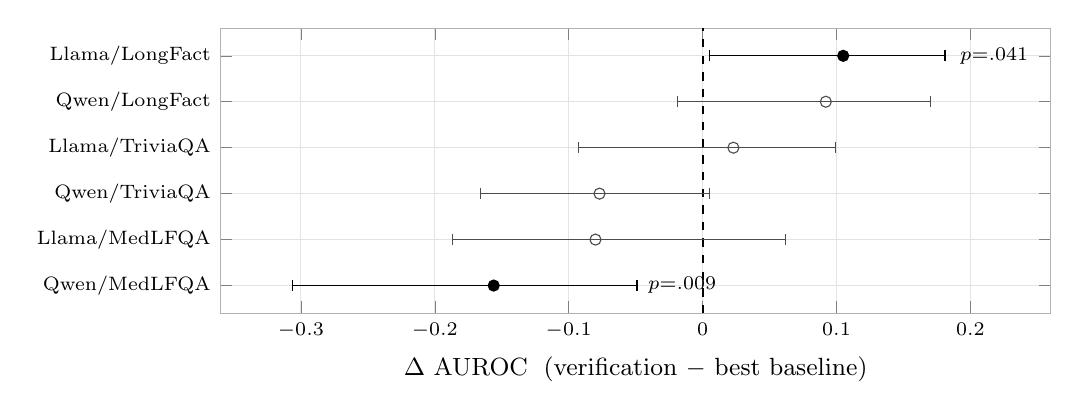
\begin{tikzpicture}
\begin{axis}[
  width=\columnwidth, height=5.2cm,
  xlabel={$\Delta$ AUROC \;(verification $-$ best baseline)},
  xmin=-0.36, xmax=0.26,
  ytick={1,2,3,4,5,6},
  yticklabels={Qwen/MedLFQA, Llama/MedLFQA, Qwen/TriviaQA, Llama/TriviaQA,
               Qwen/LongFact, Llama/LongFact},
  y tick label style={font=\scriptsize},
  x tick label style={font=\scriptsize},
  xlabel style={font=\small},
  ymin=0.4, ymax=6.6,
  grid=major, grid style={gray!22},
  axis line style={gray!60},
]
% zero line: no difference between verification and the baseline
\addplot[black, dashed, thick, forget plot] coordinates {(0,0.4) (0,6.6)};
% significant cells (95% CI excludes zero): filled markers
\addplot[only marks, mark=*, mark size=2pt, black,
         error bars/.cd, x dir=both, x explicit]
  coordinates {
    (-0.156,1) += (0.107,0) -= (0.150,0)
    ( 0.105,6) += (0.076,0) -= (0.100,0)
  };
% inconclusive cells (CI straddles zero): open markers
\addplot[only marks, mark=o, mark size=2pt, gray!60!black,
         error bars/.cd, x dir=both, x explicit]
  coordinates {
    (-0.080,2) += (0.142,0) -= (0.107,0)
    (-0.077,3) += (0.082,0) -= (0.089,0)
    ( 0.023,4) += (0.076,0) -= (0.116,0)
    ( 0.092,5) += (0.078,0) -= (0.111,0)
  };
\node[anchor=west, font=\scriptsize] at (axis cs:0.185,6) {$p{=}.041$};
\node[anchor=west, font=\scriptsize] at (axis cs:-0.048,1) {$p{=}.009$};
\end{axis}
\end{tikzpicture}
\caption{\textbf{Paired bootstrap ($B{=}10^4$) on $\Delta=$ best-verify $-$ best-baseline},
one row per cell with per-item scores. Bars are $95\%$ percentile CIs; filled markers are the
two cells whose CI excludes zero. Only Llama/LongFact is a significant \emph{win}, and
Qwen/MedLFQA is a significant \emph{loss}; the other four straddle zero and are inconclusive
rather than null. CI widths of $0.11$--$0.30$ set the resolution of this design.}
\label{fig:forest}
\end{figure}

\begin{table}[t]
\centering\small
\setlength{\tabcolsep}{3.5pt}
\begin{tabular}{lc cccccc c}
\toprule
data type & cells & $n_1$ & $n_2$ & $n_3$ & $n_4$ & $n_6$ & $n_7$ & verify \\
\midrule
General, short-form & 10 & 1 & 1 & 6 & 1 & 1 & 0 & 1/10 \\
General, long-form  &  2 & 0 & 0 & 0 & 0 & 0 & 2 & \textbf{2/2} \\
Adversarial         &  6 & 1 & 1 & 4 & 0 & 0 & 0 & \textbf{0/6} \\
Health, MCQ         &  8 & 4 & 1 & 3 & 0 & 0 & 0 & \textbf{0/8} \\
Health, free-form   &  3 & 2 & 0 & 1 & 0 & 0 & 0 & \textbf{0/3} \\
Health, long-form   &  3 & 2 & 1 & 0 & 0 & 0 & 0 & \textbf{0/3} \\
Math                &  4 & 0 & 0 & 3 & 0 & 0 & 1 & 1/4 \\
Multi-hop           &  2 & 0 & 0 & 0 & 1 & 0 & 1 & 1/2 \\
\midrule
\textbf{Total}      & \textbf{38} & 10 & 4 & 17 & 2 & 1 & 4 & \textbf{5/38} \\
\bottomrule
\end{tabular}
\caption{\textbf{Which estimator wins, by data type}, counting cells over all six targets
(38 non-degenerate model$\times$dataset cells; per-cell values in
Appendix~\ref{app:bydataset}). Read by \emph{data type} rather than by model, the structure is
sharp: verification ($n_6/n_7$) wins \textbf{both} long-form general-knowledge cells and
\textbf{none} of the fourteen health cells---indeed only $5$ of $38$ overall---while the two
baselines ($n_1$ verbalized, $n_3$ $\phi$) take $27$ of $38$. The dataset predicts the winner far better than the target
model does.}
\label{tab:groups}
\end{table}

\begin{table}[t]
\centering\small
\begin{tabular}{lccr}
\toprule
data type & cells & single-answer wins & median $\Delta$ \\
\midrule
Adversarial      & 4 & \textbf{4/4} & $+0.169$ \\
Health MCQ       & 6 & \textbf{5/6} & $+0.088$ \\
Health long-form & 3 & 1/3 & $-0.018$ \\
General long-form& 2 & 0/2 & $-0.014$ \\
Health free-form & 2 & 0/2 & $-0.026$ \\
Math             & 4 & 1/4 & $-0.072$ \\
General short-form& 8 & 1/8 & $-0.048$ \\
\midrule
\textbf{Total}   & 29 & \textbf{12/29} & \\
\bottomrule
\end{tabular}
\caption{\textbf{Single-answer vs.\ multi-sample estimators, by data type.} Each cell is one
(model, dataset) pair in which both families were run and the class balance supports an AUROC
(minority $\ge15$); ``wins'' counts cells where the best single-answer rung exceeds the best
multi-sample baseline, and $\Delta$ is their difference. Single-answer estimators dominate where
a model's errors are \emph{consistent}---adversarial content and multiple-choice---and lose where
errors are inconsistent, which is exactly where resampling has dispersion to measure. Grey-box
P(True) is excluded from the multi-sample side throughout. Per-cell values in
Appendix~\ref{app:bydataset}.}
\label{tab:family}
\end{table}

\subsection{Which family wins is decided by the data}\label{sec:family}
Table~\ref{tab:family} is the paper's central result. Aggregated over $29$ non-degenerate cells
in which both families ran, single-answer estimators win $12$---a near-even split that, taken
alone, would say little. Disaggregated by data type it is not close to even: they take
\textbf{all four} adversarial cells and \textbf{five of six} multiple-choice health cells, and
lose seven of eight general short-form cells, three of four math cells, and both general
long-form cells.

\paragraph{Adversarial content: the mechanism in its clearest form.} TruthfulQA is built from
questions whose plausible answer is a common human misconception, so a model that has absorbed
the misconception reproduces it \emph{stably}. Resampling therefore measures agreement about a
falsehood. On Llama-3.3-70B every multi-sample baseline lands between $0.492$ and $0.538$---three
of them at exactly $0.500$---while a single verbalized call reaches $0.782$, a gap of $0.28$. The
same ordering holds on all four targets where both families ran, with a median advantage of
$+0.169$ to the single-answer side. Sampling is not weak here; it is measuring the wrong quantity.

\paragraph{Multiple-choice: nothing to disperse.} On MedQA and MMLU-Med the answer is one letter.
A confidently wrong model emits the same letter every time, and the multi-sample scores collapse:
discrete semantic entropy is exactly $0.500$ on four of the six cells. Single-answer estimators
win five of six, median $+0.088$.

\paragraph{Where errors are unstable, sampling works.} The ordering reverses wherever a model's
mistakes vary between attempts. On general-knowledge short form multi-sample methods win seven of
eight cells (median $0.048$), on LongFact both, and on GSM8K three of four---arithmetic is the
clearest case of the complementary mechanism, since a model that cannot do the computation makes
a \emph{different} slip each time, and lexical similarity alone reaches $0.842$ on Llama-8B
against $0.654$ for our best rung. This is the regime the multi-sample literature was developed on, and our results reproduce
it. The cost is not free, however: on LongFact the two families are level at $N{=}5$
($0.645$/$0.699$ for the best baseline against $0.644$/$0.716$ for $n_7$) and the baselines only
pull ahead at $N{=}10$, i.e.\ ten additional generations of a $180$-word answer against the one
generation the answer already cost.

\subsection{Inside the single-answer family: no scoring rule dominates}\label{sec:minority}
Having established \emph{which family} to use, we ask which scoring rule within the
single-answer family. Table~\ref{tab:groups} aggregates the seven rungs over the full
$6\times12$ grid. No rule dominates: the two simplest---a global self-rating ($n_1$) and a
deterministic aggregation over self-rated risk ($n_3$)---take $27$ of $38$ cells between them,
and each of the remaining rungs is best somewhere; the full seven-rung ladder is in
Appendix~\ref{app:ladder} and the large-open grid in Appendix~\ref{app:bigopen}. Three patterns
are stable.

\paragraph{Verification wins long-form general knowledge, and only there.} Both LongFact cells go
to $n_7$, and they are the only cells in the study where \emph{every} self-rating rung loses to
\emph{both} discriminative rungs. The separation is complete: on LongFact the four self-rating
variants span $0.438$--$0.623$ and the two discriminative variants span $0.627$--$0.716$, with no
overlap (Appendix~\ref{app:bydataset}). Because $n_2$, $n_3$ and $n_4$ share the identical
decomposition with $n_6$ and $n_7$ and differ only in how each claim is scored, this isolates the
\emph{discriminative read} as the operative ingredient---decomposition alone buys nothing here.

\paragraph{Verification never wins on health: $0$ of $14$ cells.} Across MCQ, free-form and
long-form health, over 8B, 32B, 70B and frontier closed targets, no verification rung is ever
best; the cells split $8$/$4$/$2$ between $n_1$, $n_3$ and $n_2$. MedQA is the cleanest instance:
six targets, six losses. We read this as a property of the answer rather than the domain
alone---a multiple-choice letter has nothing to decompose, so the machinery has no purchase---but
the pattern also holds for free-form and long-form health, where the per-claim risk carries no
correctness signal (\S\ref{sec:inversion}).

\paragraph{Elsewhere the baselines win.} On short-form general knowledge, adversarial and math,
$n_3$ ($\phi$ over self-rated risk) or plain verbalized confidence is best in $19$ of $22$ cells.
Overall, the two baselines take $23$ of $38$ cells and the two verification rungs take $9$; the
blanket claim ``decomposed verification beats verbalized confidence'' is false. We also note that a rung we might have discarded, $n_2$ (per-claim
self-rated confidence), is best on four cells including the single largest margin in the grid
($+0.131$ on Llama/MMLU-Med), so the ladder's intermediate steps are not uniformly dominated.

\subsection{The exception: long-form general knowledge}\label{sec:longfact}
Table~\ref{tab:longfact} is the paper's one significant positive result. On LongFact,
self-consistency verification (\nsc) reaches $0.644$/$0.716$ against a verbalized floor of
$0.540$/$0.623$---\textbf{$+0.105$ and $+0.092$}---on two independent 8B targets, at $n{=}300$
with 61 and 41 negatives (the largest and best-balanced cells in the study). Under a paired
bootstrap the Llama effect is significant ($95\%$ CI $[+0.005,+0.181]$, $p{=}0.041$) while the
Qwen effect, though nearly the same size, is not ($p{=}0.107$); we report both rather than
pooling them, and note that a design powered to resolve a $0.09$ effect at this class balance
would need several times $300$ items. The gain is
attributable to the \emph{discriminative read} rather than to decomposition, because the
deterministic-$\phi$ rung shares the identical decomposition and does not benefit: $\phi$
scores $0.525$/$0.613$, statistically indistinguishable from the verbalized floor. We
therefore avoid the word ``collapse'' for $\phi$ on long-form; the accurate statement is that
structured self-rated risk buys nothing here, while a fresh yes/no verification buys $\sim0.10$.
Self-consistency ($n_7$) edges decision-framing ($n_6$) by $+0.017$/$+0.014$, which is inside
noise; we do not claim a difference between them, and note that $n_7$ is also the less stable
rung elsewhere (e.g.\ $0.378$ on GPT-4o/GSM8K). We also tested the multi-sample baselines here rather than assuming them impractical. They are
applicable, merely expensive: at $N{=}5$ the best of them reaches $0.645$/$0.699$, level with
\nsc\ ($0.644$/$0.716$), and at $N{=}10$ the best (MatrixDegree) reaches $0.658$/$0.747$,
\emph{ahead} of \nsc\ by $+0.014$/$+0.031$---well inside the confidence intervals of
\S\ref{sec:results}, but ahead. The honest statement is therefore not that verification is the
only option on long-form, but that it matches a $5$-sample ensemble and trails a $10$-sample one
while consuming a single target generation; on short QA, where resampling is cheap,
the spectral baseline EigV ($0.798$ on Llama/TriviaQA) still leads (Table~\ref{tab:baselines}).

\subsection{On inversion, and on the reproducibility of closed targets}\label{sec:inversion}
An earlier version of this work reported that verbalized confidence is \emph{inverted} on closed
targets---AUROC below chance, the model more confident on its wrong answers---and asked whether
verification rescues it. We withdraw that finding, and the reason is worth reporting.

We scored the closed targets twice, two days apart, through the same gateway with the same cached
answers, the same labels and the same items. The rungs $n_1$, $n_3$ and $n_6$ are greedy
($T{=}0$) and should be reproducible exactly. They were not: $12$ of $32$ paired comparisons
moved by more than $0.10$ AUROC. Both cells that carried the inversion story moved out of it---
GPT-4o/BioASQ from $0.346$ to $0.513$ and Claude/TruthfulQA from $0.484$ to $0.728$---leaving
\emph{no} valid inverted cell in the grid. No API call failed in either run (the client logs zero
give-ups), the item sets and class balances are identical, and a live probe parses cleanly, so
this is not a harness fault. The most likely explanation is that \texttt{openai/gpt-4o} and
\texttt{anthropic/claude-haiku-4.5} are \emph{aliases} that were re-pointed to newer snapshots
between the two runs.

We therefore report the second run throughout, and we draw a methodological conclusion rather
than a scientific one: \textbf{closed-target uncertainty results are not reproducible unless the
provider's snapshot identifier is pinned and recorded}. Benchmarks that report a single
closed-model number---ours included, before this check---are reporting a measurement whose
referent can change without notice. We recommend that pure-black-box evaluations record the
resolved model version with every cell, and we release both runs so the discrepancy can be
inspected.

What survives is a cleaner negative result about the closed targets. In the second run
$\phi$ ($n_3$) is the best estimator on six of the seven valid closed cells ($0.612$--$0.780$),
and verification wins \emph{none} of them. Together with $0/4$ on Qwen3-32B and $0/5$ on
Llama-3.3-70B, all five of verification's wins in the grid occur on the two 8B targets.

\subsection{The latency trade}
\begin{table}[t]
\centering\small
\begin{tabular}{llcccc}
\toprule
Target & Dataset & \nverb & \nphi & \nyn & \nsc \\
\midrule
Llama & TriviaQA & 259 & 4469 & 1440 & 2299 \\
Llama & LongFact & 270 & 23639 & 10858 & 18831 \\
Llama & MedLFQA  & 183 & 5656 & 3719 & 6964 \\
\midrule
Qwen  & TriviaQA & 286 & 7576 & 1462 & 2474 \\
Qwen  & LongFact & 308 & 15656 & 8076 & 12641 \\
Qwen  & MedLFQA  & 284 & 7672 & 1717 & 2721 \\
\bottomrule
\end{tabular}
\caption{\textbf{Median per-item latency (ms).} Verbalized (\nverb) is one short call.
On long-form, discriminative verification (\nyn/\nsc) is both \emph{more accurate and
faster} than $\phi$-CoI (\nphi), which must emit a large multi-claim JSON object.
Self-consistency (\nsc) costs $\sim$1.5$\times$ decision-framing (\nyn).}
\label{tab:latency}
\end{table}
Latency (Table~\ref{tab:latency}) makes the case sharper. On LongFact, $\phi$-CoI is the
slowest estimator ($16$--$24$s/item) because it emits a large structured object per
answer; the verification rungs produce tiny yes/no completions and run at $8$--$19$s while
scoring higher. Thus on long-form general knowledge the verification rungs
\textbf{dominate $\phi$-CoI on both axes} (full latency grid, Appendix~\ref{app:latency}).
Verbalized confidence remains far cheaper
($\sim$0.3s) and is the right choice when its lower accuracy is acceptable; self-consistency
buys ${\approx}0.10$ AUROC at a $41$--$70\times$ latency cost over the single call on LongFact
(the ratio is smaller on shorter datasets; full grid in Appendix~\ref{app:latency}).

\begin{table}[t]
\centering\small
\begin{tabular}{llccccc}
\toprule
Target & Dataset & neg. & \nverb & \nphi & \nyn & \nsc \\
\midrule
\multirow{4}{*}{GPT-4o}
 & TriviaQA   & 24 & 0.512 & 0.500 & 0.525 & \textbf{0.535} \\
 & TruthfulQA & 40 & 0.508 & 0.511 & \textbf{0.530} & 0.513 \\
 & MedQA      & 16 & \textbf{0.591} & 0.545 & 0.471 & 0.521 \\
 & BioASQ     & 38 & 0.346 & \textbf{0.622} & 0.457 & 0.466 \\
\cmidrule(l){2-7}
 & \grey{MedLFQA}  & \grey{7} & \grey{0.337} & \grey{0.487} & \grey{0.524} & \grey{0.675} \\
 & \grey{GSM8K}    & \grey{6} & \grey{0.601} & \grey{0.495} & \grey{0.643} & \grey{0.378} \\
\midrule
\multirow{3}{*}{Claude-H}
 & TriviaQA   & 32 & 0.514 & 0.571 & \textbf{0.588} & 0.569 \\
 & TruthfulQA & 27 & 0.484 & 0.510 & 0.498 & \textbf{0.596} \\
 & MedQA      & 19 & 0.527 & \textbf{0.658} & 0.510 & 0.504 \\
\cmidrule(l){2-7}
 & \grey{MedLFQA}  & \grey{8} & \grey{0.469} & \grey{0.400} & \grey{0.387} & \grey{0.593} \\
 & \grey{GSM8K}    & \grey{4} & \grey{0.837} & \grey{0.728} & \grey{0.422} & \grey{0.527} \\
\bottomrule
\end{tabular}
\caption{\textbf{Closed-target grid} (AUROC; ``neg.'' is the minority-class count). Rows below
each rule are \textbf{degenerate} (minority $<15$): they are shown in grey for transparency and
excluded from every claim and from the win-rates in Table~\ref{tab:winrate}. Among valid cells verification wins
$0/4$ (GPT-4o) and $0/3$ (Claude): $\phi$ is best on six of the seven, at $0.612$--$0.780$.
These are the second-run values; the first run gave systematically different numbers on the same
greedy estimators, which we report as a reproducibility finding in \S\ref{sec:inversion}.}
\label{tab:closed}
\end{table}

\subsection{Supporting grids and baselines}
The full 8B suite (Appendix~\ref{app:suite}, Table~\ref{tab:suite}) shows the pattern in
detail: verification wins LongFact, HotpotQA and (Llama) GSM8K, while short-factual, MCQ,
and most health cells go to \nverb\ or \nphi. On the open 8B \emph{and} large targets, MedLFQA
verbalized confidence stays informative and is the best pure black-box signal of any kind---it
beats even the multi-sample baselines (Table~\ref{tab:baselines}: best baseline EigV
$0.62$/$0.53$). Chain inspection explains the open-model behavior: on MedLFQA the 8B per-claim
self-rated risk is uninformative (mean risk $0.385$ for both correct and incorrect answers) and
grounding is a near-constant---so $\phi$ collapses, while a \emph{holistic} verbalized judgment
still separates. On the closed targets the same ordering holds and is if anything sharper: $\phi$ is best on six
of seven valid cells, and neither discriminative rung wins any. The multi-sample baselines (Table~\ref{tab:baselines}) confirm the regime split:
strong on short QA (they resample the target $N{=}5\times$), and competitive on long-form
only once $N{=}10$ full resamples are paid.

\begin{table}[t]
\centering\small
\begin{tabular}{llccc}
\toprule
Target & Dataset & DSE & LexSim & EigV \\
\midrule
Llama-8B & TriviaQA & 0.750 & 0.760 & \textbf{0.798} \\
Llama-8B & MedLFQA  & 0.513 & 0.582 & 0.623 \\
Llama-8B & LongFact & 0.553 & 0.531 & 0.640 \\
Qwen-8B  & TriviaQA & 0.686 & 0.715 & 0.688 \\
Qwen-8B  & MedLFQA  & 0.524 & 0.484 & 0.526 \\
Qwen-8B  & LongFact & 0.592 & 0.592 & 0.708 \\
\bottomrule
\end{tabular}
\caption{\textbf{Multi-sample baselines} (AUROC, $N{=}5$, 3-seed means): discrete semantic
entropy, lexical similarity, graph-Laplacian spectral (EigV). They resample the target
$5\times$ (so cost $5\times$ the answer, against one generation for our single-answer rungs). Strong on short QA; near chance on MedLFQA---where single-call verbalized confidence
($0.647$/$0.678$, Table~\ref{tab:suite}) beats them. \textbf{LongFact values are new to this
work}: rather than assume these methods impractical on long-form, we paid the cost
($10$ resampled $180$-word answers per item, ${\approx}37$\,min of generation per target) and
report what they achieve; see \S\ref{sec:longfact}. Short-form rows are 3-seed means whereas our
rungs are single-seed, so that comparison is not symmetric (Limitations).}
\label{tab:baselines}
\end{table}

\subsection{Can better aggregation math rescue $\phi$?}
Because $\phi$'s weakness on long-form is an aggregation of per-claim scores, we asked
whether a better aggregator recovers signal. Offline, over the cached CoI features, we
compared the fixed-prior $\phi$ against closed-form pools (mean/max/product of
$1{-}r$; grounding-weighted min/mean) and a cross-validated logistic regression fit on
$13$ CoI features (Appendix~\ref{app:agg}). \textbf{No aggregator improves on the fixed prior
by more than sampling error.} Differences run in both directions and are all small:
a min-pool of $\mathrm{base}\cdot(1{-}r)$ is nominally ahead on Llama/TriviaQA ($0.711$ vs.\
$\phi$'s $0.686$) while the cross-validated logistic regression is nominally behind on
Qwen/MedLFQA ($0.631$ vs.\ $0.657$); none of these gaps is resolvable at $n{\approx}150$.
Notably the learned aggregator, despite $13$ features, never pulls clear of a fixed prior with
no training data at all. And on MedLFQA every aggregator sits near $0.50$. The lesson is that
the aggregator is not the bottleneck; the \emph{inputs} (self-rated risk) are, which is
precisely what the verification rungs replace.

\section{Discussion}\label{sec:discussion}
The practical rule that follows is about \emph{families} first and scoring rules second.
Multi-sample estimation is the right default on general-knowledge content, short or long, where a
model's errors are unstable enough for dispersion to detect them---and where the extra
generations buy roughly $0.05$ AUROC. It should \emph{not} be the default on adversarial or
multiple-choice content, where a wrong answer is reproduced reliably and dispersion measures
agreement about the error: there a single-answer estimator is both better (median $+0.169$ and
$+0.088$) and free, since the answer has already been generated. The diagnostic is available
before deployment---if resampling a held-out set produces near-identical answers on the errors,
sampling-based uncertainty cannot work on that content.

Within the single-answer family we do not recommend a specific rung. Decomposed verification
earns its cost only on long-form answers, and even there it is level with a $5$-sample ensemble;
elsewhere a single verbalized call or the deterministic $\phi$ is as good or better and far
cheaper.

We had expected a second regime, \textbf{overconfident targets}, where a below-chance verbalized
AUROC signals that the self-rating is anti-correlated with correctness. Our data cannot support
that claim (\S\ref{sec:inversion}), and we flag two reasons it remains attractive but unproven.
First, the obvious control is unfavourable: if verbalized confidence is \emph{reliably}
inverted, negating it is a one-call fix. In the run we now report there is no valid inverted
cell at all, so the question does not arise; the earlier finding rested on scores we can no
longer reproduce (\S\ref{sec:inversion}). Second, ``inverted'' and ``closed-weights'' are perfectly
confounded in this grid. A deployable router of the form ``measure verbalized reliability on
held-out data, escalate where it is poor'' is therefore a hypothesis our results motivate but do
not establish; testing it needs inverted open targets and long-form closed cells with adequate
class balance.

\section{Conclusion}
Multi-sample uncertainty estimation assumes a model's errors are unstable enough to show up as
disagreement among resamples. We show that assumption is a property of the \emph{data}, not of
the method, and that it fails predictably. Across six targets and twelve datasets, single-answer
estimators---which score the one answer already generated and pay nothing extra---beat
multi-sample consistency and spectral baselines on \textbf{all four} adversarial cells (median
$+0.169$) and \textbf{five of six} multiple-choice health cells (median $+0.088$), because
imitative falsehoods and confidently wrong options are reproduced identically on every resample.
On general-knowledge content, where errors are unstable, the ordering reverses and multi-sample
methods win $7$ of $8$ short-form cells and both long-form cells---though on long-form only at
$N{=}10$, ten extra generations of the answer against the single one it already cost.

Within the single-answer family we ablate seven scoring rules and find no universal winner: a
global self-rating and a deterministic aggregation over self-rated risk take $23$ of $38$ cells
between them, and discriminative verification earns its cost only on long-form. Paired bootstrap
intervals show that many differences \emph{within} the family are not resolvable at these sample
sizes, so we offer a selection rule between families rather than a new estimator. We release the
harness, every per-item score, and the per-cell class balances needed to check these claims.

\section*{Limitations}
Our closed-target numbers are a snapshot, not a stable measurement. We scored GPT-4o and
Claude-Haiku twice through the same gateway two days apart and $12$ of $32$ greedy comparisons
moved by more than $0.10$ AUROC, which removed an inversion finding we had drawn from the first
run. We report the second run and release both, but a third run could differ again, and no
closed-target claim here should be treated as more precise than that.
\paragraph{Statistical power.} Every CoI number is \emph{single-seed}, while the multi-sample
baselines we quote are 3-seed means---so Table~\ref{tab:baselines} is not a symmetric
comparison. The 8B cells use seed 1 and the large-open and closed cells seed 0, so the two
halves of the grid do not even share a seed. We have no seed variance, and at $n{\approx}150$
we therefore ran a paired bootstrap ($B{=}10^4$, resamples shared across rungs) on the six
cells for which we retain per-item scores (Appendix~\ref{app:boot}). It is sobering: $95\%$ CI
widths are $0.11$--$0.30$ AUROC, so this design can only resolve differences of roughly $0.15$
and above. Exactly one positive effect is significant (Llama/LongFact, $p{=}0.041$) and one
negative effect is (Qwen/MedLFQA, $p{=}0.009$); every other comparison we report, including the
Qwen LongFact gain of $+0.092$ ($p{=}0.107$), is inconclusive at this sample size. Readers
should treat the per-cell orderings in Tables~\ref{tab:suite}--\ref{tab:closed} as descriptive.
We could not bootstrap the large-open or closed cells, whose per-item scores were not retained;
their CIs would be no narrower.

\paragraph{Class balance and excluded cells.} We exclude cells whose minority class is $<15$.
This removes BioASQ on all open targets (as few as one negative) and both closed MedLFQA and
GSM8K cells (4--8 negatives). Those closed cells are exactly where a clean
``verification rescues overconfidence'' story would have lived, so its absence is a limitation
of the data, not evidence against the hypothesis. Per-cell counts are in
Table~\ref{tab:stats} for the 8B targets and in Table~\ref{tab:closed} for the closed arm.

\paragraph{Coverage and confounds.} The large-open and closed targets are evaluated on the six
datasets with cached generations, not the full twelve, so LongFact and multi-hop are measured
only on 8B. The long-form and overconfidence conditions therefore never co-occur in a single
non-degenerate cell. Moreover every inverted target in our grid is closed and every calibrated
one is open, so inversion and closed-weights are collinear and we cannot attribute the effect to
either. We make no claim about inverted baselines: the two cells that were inverted in our first run are
not inverted in the run we report, and we could not reproduce closed-target scores across
provider snapshots (\S\ref{sec:inversion}).

\paragraph{Labels.} Correctness comes from an LLM judge (Qwen3-4B; letter-match for MCQ) that we
did not validate against human annotation, and LongFact factuality from a 70B judge without
retrieval---parametric factuality, not ground truth. Absolute AUROCs inherit that noise; we rely
on relative orderings within a cell, where judge error is at least shared across estimators.

\paragraph{Calibration.} Verification's ECE (Table~\ref{tab:ece}, Appendix~\ref{app:ece}) is worse than verbalized
confidence in raw scale because votes are coarse. Discrimination (AUROC) is our headline and
post-hoc calibration is orthogonal, but a deployed router would need calibrated scores.

\section*{Ethics Statement}
Four of our datasets are medical (MedQA, MMLU-Med, BioASQ, K-QA, MedLFQA) and the deployment
story we discuss---gating or escalating answers by a confidence score---would, in a health
setting, decide which model outputs reach a person. We report that no estimator we tested is
reliable on health long-form: the best AUROC is around $0.65$, and on several health cells every
method is near chance. A confidence signal at that level must not be used to suppress review of
medical content, and we explicitly do not recommend deploying these estimators as a safety gate
in clinical or patient-facing settings. All datasets are public and used under their licenses;
no human-subjects data was collected and no annotation was crowdsourced for this work.

% ---- CAMERA-READY ONLY: de-anonymizing; restore after acceptance ----
% \section*{Acknowledgments}
% This work was done in part at the 2026 Jelinek Memorial Summer Workshop on Speech and
% Language Technology and was supported by NSF CCRI Grant No.\ 2120435, Google DeepMind, the
% JHU Amazon Initiative for Interactive Artificial Intelligence, the JHU Human Language
% Technology Center of Excellence, and the Association for Computational Linguistics.

\bibliographystyle{acl_natbib}
\bibliography{references}

\appendix
\section{Full ablation ladder ($n{=}1$--$7$)}\label{app:ladder}
The main text reports the four informative rungs ($n_1,n_3,n_6,n_7$). Table~\ref{tab:ladder}
gives all seven, on the two cells where every rung was run. Two clarifications. First, \textbf{$n_5$ is not an independent rung}: it issues the same chain
prompt as $n_4$ and adds a final self-rating that is \emph{logged but never scored}, so its
reported score is $\phi$ and is identical to $n_4$ by construction---exactly so in all four
cells ($0.688$, $0.618$, $0.732$, $0.686$). We keep the column for completeness but it measures
nothing beyond $n_4$ while costing $2.2\times$ the latency ($12.6$\,s vs.\ $5.8$\,s on TriviaQA,
$14.8$\,s vs.\ $6.8$\,s on MedLFQA), so it is strictly dominated; the $n_4{\to}n_5$ comparison
should not be read as an ablation.
Second, the intermediate rungs are dominated \emph{on average} but not everywhere: $n_2$
(per-claim self-rated confidence) is the outright best estimator on Qwen/MedLFQA at $0.709$,
ahead of $n_1$, $n_3$ and both verification rungs---a health long-form cell we otherwise report
as a loss for decomposition. Nor is $n_4$ (separate evidence and critique chains) uniformly
close to $n_3$: it is $+0.002$ on Llama/TriviaQA but $+0.117$ on Llama/MedLFQA, $+0.030$ on
Qwen/MedLFQA and $-0.057$ on Qwen/TriviaQA. Splitting the critique into its own pass therefore
helps precisely on the health long-form cells where the single-pass $\phi$ collapses, which is
the one place we might have wanted it to. We do not build on this---the differences are inside
the confidence intervals of \S\ref{sec:results} and rest on two cells---but it is the most
promising unexplored direction in the ladder, and we flag it rather than bury it. Splitting or re-rating the chain does not help; only the discriminative read
($n_6/n_7$) or, on short QA, $n_3$ moves the needle. This is why we carry $\{n_1,n_3,n_6,n_7\}$
forward as the representative ladder.
\begin{table}[t]
\centering\small
\setlength{\tabcolsep}{3.5pt}
\begin{tabular}{llccccccc}
\toprule
Target & Data & $n_1$ & $n_2$ & $n_3$ & $n_4$ & $n_5$ & $n_6$ & $n_7$ \\
\midrule
Llama-8B & TriviaQA & 0.659 & 0.662 & 0.686 & 0.688 & 0.688 & \textbf{0.709} & 0.661 \\
Llama-8B & MedLFQA  & \textbf{0.647} & 0.563 & 0.500 & 0.618 & 0.618 & 0.561 & 0.567 \\
Qwen-8B  & TriviaQA & 0.727 & 0.719 & \textbf{0.790} & 0.732 & 0.732 & 0.692 & 0.713 \\
Qwen-8B  & MedLFQA  & 0.678 & \textbf{0.709} & 0.657 & 0.686 & 0.686 & 0.492 & 0.521 \\
\bottomrule
\end{tabular}
\caption{\textbf{Full ablation ladder}, AUROC. $n_1$ verbalized; $n_2$ per-claim self-rated
confidence; $n_3$ deterministic $\phi$ over self-rated risk; $n_4$ separate evidence/critique
chains; $n_5$ adds a final self-rating that is logged but not scored, so its reported value is $\phi$ and coincides with $n_4$ exactly; $n_6$ decision-framed
verify; $n_7$ self-consistency verify.}
\label{tab:ladder}
\end{table}

\section{Large open targets (32B/70B)}\label{app:bigopen}
Table~\ref{tab:bigopen} gives the AUROC grid for the strong open targets (4-bit), on the six
datasets with cached generations. Verification ($n_6/n_7$) wins none of these cells: $\phi$
($n_3$) leads on general/adversarial/math, and verbalized ($n_1$) on the health cells. MedLFQA
stays above chance for Llama-70B ($0.635$, $n_1$) and is degenerate for Qwen-32B---the contrast
with the closed-target reproducibility check (Table~\ref{tab:inversion}) is examined in
\S\ref{sec:results}.
\begin{table}[t]
\centering\small
\begin{tabular}{llcccc}
\toprule
Target & Dataset & \nverb & \nphi & \nyn & \nsc \\
\midrule
\multirow{5}{*}{Qwen3-32B}
 & TriviaQA   & 0.685 & \textbf{0.777} & 0.545 & 0.628 \\
 & TruthfulQA & 0.748 & \textbf{0.759} & 0.662 & 0.701 \\
 & MedQA      & 0.705 & \textbf{0.772} & 0.533 & 0.609 \\
 & \grey{MedLFQA} & \grey{0.510} & \grey{0.437} & \grey{0.489} & \grey{0.486} \\
 & GSM8K      & 0.769 & \textbf{0.815} & 0.563 & 0.631 \\
\midrule
\multirow{5}{*}{Llama-3.3-70B}
 & TriviaQA   & 0.656 & \textbf{0.684} & 0.660 & 0.675 \\
 & TruthfulQA & \textbf{0.782} & 0.771 & 0.582 & 0.590 \\
 & MedQA      & \textbf{0.673} & 0.574 & 0.568 & 0.603 \\
 & MedLFQA    & \textbf{0.635} & 0.477 & 0.553 & 0.547 \\
 & GSM8K      & 0.610 & \textbf{0.623} & 0.557 & 0.540 \\
\bottomrule
\end{tabular}
\caption{\textbf{Large open targets} (AUROC, 4-bit, seed 0; BioASQ degenerate, omitted).
Verification wins $0/9$ valid cells: strong open judges keep $\phi$/verbalized informative
(the Qwen3-32B MedLFQA row is degenerate and excluded from the count).}
\label{tab:bigopen}
\end{table}

\section{ECE by rung}\label{app:ece}
\begin{table}[t]
\centering\small
\begin{tabular}{llcccc}
\toprule
Target & Dataset & \nverb & \nphi & \nyn & \nsc \\
\midrule
\multirow{7}{*}{Llama-8B}
 & TriviaQA   & 0.186 & 0.109 & 0.300 & 0.237 \\
 & LongFact   & 0.143 & 0.240 & 0.417 & 0.344 \\
 & TruthfulQA & 0.285 & 0.082 & 0.244 & 0.235 \\
 & MedQA      & 0.245 & 0.189 & 0.238 & 0.201 \\
 & MedLFQA    & 0.104 & 0.262 & 0.366 & 0.334 \\
 & GSM8K      & 0.221 & 0.174 & 0.491 & 0.518 \\
 & HotpotQA   & 0.261 & 0.262 & 0.361 & 0.245 \\
\midrule
\multirow{7}{*}{Qwen-8B}
 & TriviaQA   & 0.389 & 0.107 & 0.315 & 0.302 \\
 & LongFact   & 0.080 & 0.207 & 0.160 & 0.149 \\
 & TruthfulQA & 0.294 & 0.083 & 0.327 & 0.308 \\
 & MedQA      & 0.171 & 0.155 & 0.413 & 0.391 \\
 & MedLFQA    & 0.053 & 0.263 & 0.127 & 0.121 \\
 & GSM8K      & 0.099 & 0.075 & 0.393 & 0.366 \\
 & HotpotQA   & 0.478 & 0.141 & 0.260 & 0.235 \\
\bottomrule
\end{tabular}
\caption{Expected calibration error (lower better), 8B targets. Verification rungs
discriminate well (Tables~\ref{tab:longfact}, \ref{tab:suite}) but are less calibrated in raw
scale (coarse votes); $\phi$ ($n_3$) is best-calibrated. Post-hoc calibration is orthogonal to
the AUROC result and would be applied per (target,domain) at deployment.}
\label{tab:ece}
\end{table}

\section{Full 8B dataset suite}\label{app:suite}
\begin{table}[t]
\centering\small
\setlength{\tabcolsep}{4pt}
\begin{tabular}{llcccc}
\toprule
Target & Dataset & \nverb & \nphi & \nyn & \nsc \\
\midrule
\multirow{11}{*}{Llama-3.1-8B}
 & TriviaQA   & 0.659 & 0.686 & \textbf{0.709} & 0.661 \\
 & NaturalQA  & \textbf{0.726} & 0.671 & 0.613 & 0.615 \\
 & PopQA      & 0.500 & \textbf{0.780} & 0.479 & 0.479 \\
 & LongFact   & 0.540 & 0.525 & 0.627 & \textbf{0.644} \\
 & TruthfulQA & 0.671 & \textbf{0.677} & 0.621 & 0.560 \\
 & MedQA      & \textbf{0.568} & 0.551 & 0.567 & 0.563 \\
 & MMLU-Med   & 0.555 & \textbf{0.570} & 0.467 & 0.390 \\
 & K-QA       & \textbf{0.632} & 0.592 & 0.544 & 0.618 \\
 & MedLFQA    & \textbf{0.647} & 0.500 & 0.561 & 0.567 \\
 & GSM8K      & 0.639 & 0.554 & 0.619 & \textbf{0.654} \\
 & HotpotQA   & \textbf{0.752} & 0.642 & 0.489 & 0.558 \\
\midrule
\multirow{11}{*}{Qwen3-8B}
 & TriviaQA   & 0.727 & \textbf{0.790} & 0.692 & 0.713 \\
 & NaturalQA  & \textbf{0.687} & 0.621 & 0.591 & 0.612 \\
 & PopQA      & 0.643 & \textbf{0.685} & 0.617 & 0.648 \\
 & LongFact   & 0.623 & 0.613 & 0.702 & \textbf{0.716} \\
 & TruthfulQA & 0.755 & \textbf{0.769} & 0.663 & 0.678 \\
 & MedQA      & \textbf{0.739} & 0.732 & 0.641 & 0.658 \\
 & MMLU-Med   & \textbf{0.710} & 0.708 & 0.634 & 0.654 \\
 & K-QA       & 0.642 & \textbf{0.645} & 0.537 & 0.532 \\
 & MedLFQA    & \textbf{0.678} & 0.657 & 0.492 & 0.521 \\
 & GSM8K      & 0.674 & \textbf{0.726} & 0.544 & 0.530 \\
 & HotpotQA   & 0.756 & 0.703 & 0.746 & \textbf{0.766} \\
\bottomrule
\end{tabular}
\caption{\textbf{Full 8B suite} (AUROC; 150 items/cell, seed 1; BioASQ omitted as
degenerate). Verification (\nyn/\nsc) wins LongFact, HotpotQA and Llama/GSM8K; short-factual,
MCQ, adversarial and most health cells go to verbalized (\nverb) or $\phi$ (\nphi). Two cells
read exactly $0.500$ (Llama/PopQA at \nverb, Llama/MedLFQA at \nphi): the estimator returned a
constant on those cells, so the value reflects an uninformative output rather than a
graded-but-weak one.}
\label{tab:suite}
\end{table}

\section{Latency (full 8B grid)}\label{app:latency}
Table~\ref{tab:latfull} gives median per-item latency for all 8B cells. Verbalized ($n_1$) is a
single short call ($\sim$0.3\,s). $\phi$ ($n_3$) emits a full multi-claim JSON object and is the
slowest ($4.5$--$24$\,s), worst on long-form. Verification produces tiny yes/no completions:
$n_6$ is $1$--$11$\,s and $n_7$ ($K{=}5$) is $\sim$1.5--2$\times$ $n_6$. Where verification wins
(long-form), it is also \emph{faster} than $\phi$.
\begin{table}[t]
\centering\small
\setlength{\tabcolsep}{4pt}
\begin{tabular}{llrrrr}
\toprule
Target & Dataset & \nverb & \nphi & \nyn & \nsc \\
\midrule
\multirow{7}{*}{Llama-8B}
 & TriviaQA & 259 & 4469 & 1440 & 2299 \\
 & LongFact & 270 & 23639 & 10858 & 18831 \\
 & TruthfulQA & 258 & 5391 & 3280 & 5761 \\
 & MedQA & 265 & 4474 & 5523 & 10176 \\
 & MedLFQA & 183 & 5656 & 3719 & 6964 \\
 & GSM8K & 267 & 14165 & 4730 & 9073 \\
 & HotpotQA & 260 & 5616 & 2349 & 4001 \\
\midrule
\multirow{7}{*}{Qwen-8B}
 & TriviaQA & 286 & 7576 & 1462 & 2474 \\
 & LongFact & 308 & 15656 & 8076 & 12641 \\
 & TruthfulQA & 295 & 7538 & 1668 & 2707 \\
 & MedQA & 300 & 8711 & 994 & 1335 \\
 & MedLFQA & 284 & 7672 & 1717 & 2721 \\
 & GSM8K & 321 & 9808 & 1476 & 2508 \\
 & HotpotQA & 285 & 8298 & 1954 & 2963 \\
\bottomrule
\end{tabular}
\caption{Median per-item latency (ms), 8B targets, batch 1, GPU warm.}
\label{tab:latfull}
\end{table}

\section{Dataset statistics}\label{app:stats}
\begin{table}[t]
\centering\small
\begin{tabular}{lccc}
\toprule
Dataset & $n$ items & pos (Llama) & pos (Qwen) \\
\midrule
TriviaQA & 149 & 106 & 65 \\
NaturalQA & 150 & 103 & 76 \\
PopQA & 127 & 59 & 57 \\
LongFact & 300 & 239 & 259 \\
TruthfulQA & 150 & 78 & 79 \\
MedQA & 150 & 101 & 101 \\
MMLU-Med & 150 & 100 & 106 \\
BioASQ$^\dagger$ & 150 & 150 & 149 \\
K-QA & 146 & 106 & 112 \\
MedLFQA & 150 & 115 & 133 \\
GSM8K & 150 & 118 & 135 \\
HotpotQA & 150 & 45 & 51 \\
\bottomrule
\end{tabular}
\caption{Item counts and positive (correct) counts per 8B target. $^\dagger$BioASQ is
near-single-class (minority $\le 1$) and excluded from AUROC as degenerate. Positives are the
LLM-judge (or letter-match, MCQ) correct labels; LongFact uses the 70B factuality judge.}
\label{tab:stats}
\end{table}

\section{Full grid: every model $\times$ dataset $\times$ method}\label{app:bydataset}
Table~\ref{tab:bydataset} is the complete result set behind Table~\ref{tab:groups}: AUROC for
every rung on every (model, dataset) cell, grouped by data type. Best per row in bold. ``--''
means the rung was not run on that cell ($n_2$/$n_4$ were run only on the open 8B targets, where
all twelve datasets are available); degenerate cells (minority class $<15$) are greyed and
excluded from every count. The table is generated directly from the released result files by
\texttt{scripts/coi\_final\_table.py}, so the numbers here and in the body cannot drift apart.
As an independent check we also recomputed every AUROC \emph{from the raw per-item data}---the
per-item estimator outputs in the rung logs against the per-item correctness labels---rather than
re-using the values written at scoring time: all $188$ recomputable (model, dataset, rung) cells
agree to within $5\times10^{-4}$, with no mismatches
(\texttt{scripts/coi\_verify\_from\_raw.py}).

\begin{table*}[t]
\centering\small
\setlength{\tabcolsep}{5pt}
\begin{tabular}{ll cccccc}
\toprule
dataset & model & $n_1$ verb. & $n_2$ claim-conf & $n_3$ $\phi$ & $n_4$ split & $n_6$ decision & $n_7$ self-cons. \\
\midrule
% ===== General, short-form =====
TriviaQA & Llama-8B & 0.659 & 0.662 & 0.686 & 0.688 & \textbf{0.709} & 0.661 \\
 & Qwen-8B & 0.727 & 0.719 & \textbf{0.790} & 0.732 & 0.692 & 0.713 \\
 & Qwen-32B & 0.685 & -- & \textbf{0.777} & -- & 0.545 & 0.628 \\
 & Llama-70B & 0.656 & -- & \textbf{0.684} & -- & 0.660 & 0.675 \\
 & GPT-4o & 0.605 & -- & \textbf{0.780} & -- & 0.669 & 0.625 \\
 & Claude-H & 0.618 & -- & \textbf{0.755} & -- & 0.554 & 0.682 \\
\addlinespace
NaturalQA & Llama-8B & \textbf{0.726} & 0.618 & 0.671 & 0.634 & 0.613 & 0.615 \\
 & Qwen-8B & 0.687 & \textbf{0.696} & 0.621 & 0.619 & 0.591 & 0.612 \\
\addlinespace
PopQA & Llama-8B & 0.500 & 0.504 & \textbf{0.780} & 0.640 & 0.479 & 0.479 \\
 & Qwen-8B & 0.643 & 0.627 & 0.685 & \textbf{0.712} & 0.617 & 0.648 \\
\addlinespace
% ===== General, long-form =====
LongFact & Llama-8B & 0.540 & 0.469 & 0.525 & 0.438 & 0.627 & \textbf{0.644} \\
 & Qwen-8B & 0.623 & 0.601 & 0.613 & 0.555 & 0.702 & \textbf{0.716} \\
\addlinespace
% ===== Adversarial =====
TruthfulQA & Llama-8B & 0.671 & \textbf{0.738} & 0.677 & 0.662 & 0.621 & 0.560 \\
 & Qwen-8B & 0.755 & 0.715 & \textbf{0.769} & 0.732 & 0.663 & 0.678 \\
 & Qwen-32B & 0.748 & -- & \textbf{0.759} & -- & 0.662 & 0.701 \\
 & Llama-70B & \textbf{0.782} & -- & 0.771 & -- & 0.582 & 0.590 \\
 & GPT-4o & 0.557 & -- & \textbf{0.612} & -- & 0.532 & 0.466 \\
 & Claude-H & 0.728 & -- & \textbf{0.775} & -- & 0.502 & 0.668 \\
\addlinespace
% ===== Health, multiple-choice =====
MedQA & Llama-8B & \textbf{0.568} & 0.538 & 0.551 & 0.556 & 0.567 & 0.563 \\
 & Qwen-8B & \textbf{0.739} & 0.504 & 0.732 & 0.618 & 0.641 & 0.658 \\
 & Qwen-32B & 0.705 & -- & \textbf{0.772} & -- & 0.533 & 0.609 \\
 & Llama-70B & \textbf{0.673} & -- & 0.574 & -- & 0.568 & 0.603 \\
 & GPT-4o & 0.619 & -- & \textbf{0.703} & -- & 0.496 & 0.667 \\
 & Claude-H & 0.576 & -- & \textbf{0.689} & -- & 0.549 & 0.548 \\
\addlinespace
MMLU-Med & Llama-8B & 0.555 & \textbf{0.701} & 0.570 & 0.653 & 0.467 & 0.390 \\
 & Qwen-8B & \textbf{0.710} & 0.689 & 0.708 & 0.691 & 0.634 & 0.654 \\
\addlinespace
% ===== Health, free-form =====
BioASQ & \grey{Llama-8B} & \multicolumn{6}{c}{\grey{degenerate (minority 0)}} \\
 & \grey{Qwen-8B} & \multicolumn{6}{c}{\grey{degenerate (minority 1)}} \\
 & \grey{Qwen-32B} & \multicolumn{6}{c}{\grey{degenerate (minority 0)}} \\
 & \grey{Llama-70B} & \multicolumn{6}{c}{\grey{degenerate (minority 1)}} \\
 & GPT-4o & \textbf{0.513} & -- & 0.485 & -- & 0.413 & 0.448 \\
\addlinespace
K-QA & Llama-8B & \textbf{0.632} & 0.527 & 0.592 & 0.529 & 0.544 & 0.618 \\
 & Qwen-8B & 0.642 & 0.616 & \textbf{0.645} & 0.599 & 0.537 & 0.532 \\
\addlinespace
% ===== Health, long-form =====
MedLFQA & Llama-8B & \textbf{0.647} & 0.563 & 0.500 & 0.618 & 0.561 & 0.567 \\
 & Qwen-8B & 0.678 & \textbf{0.709} & 0.657 & 0.686 & 0.492 & 0.521 \\
 & \grey{Qwen-32B} & \multicolumn{6}{c}{\grey{degenerate (minority 11)}} \\
 & Llama-70B & \textbf{0.635} & -- & 0.477 & -- & 0.553 & 0.547 \\
 & \grey{GPT-4o} & \multicolumn{6}{c}{\grey{degenerate (minority 7)}} \\
\addlinespace
% ===== Math =====
GSM8K & Llama-8B & 0.639 & 0.581 & 0.554 & 0.643 & 0.619 & \textbf{0.654} \\
 & Qwen-8B & 0.674 & 0.521 & \textbf{0.726} & 0.668 & 0.544 & 0.530 \\
 & Qwen-32B & 0.769 & -- & \textbf{0.815} & -- & 0.563 & 0.631 \\
 & Llama-70B & 0.610 & -- & \textbf{0.623} & -- & 0.557 & 0.540 \\
 & \grey{GPT-4o} & \multicolumn{6}{c}{\grey{degenerate (minority 6)}} \\
\addlinespace
% ===== Multi-hop =====
HotpotQA & Llama-8B & 0.752 & 0.610 & 0.642 & \textbf{0.770} & 0.489 & 0.558 \\
 & Qwen-8B & 0.756 & 0.732 & 0.703 & 0.740 & 0.746 & \textbf{0.766} \\
\addlinespace

\bottomrule
\end{tabular}
\caption{\textbf{Complete AUROC grid} by data type, all six targets. Verification ($n_6$/$n_7$)
is best on both LongFact cells and on no health cell; see Table~\ref{tab:groups} for the
aggregate.}
\label{tab:bydataset}
\end{table*}

\section{Paired bootstrap confidence intervals}\label{app:boot}
For the six cells where we retain per-item scores (the rung raw logs), we resample items with
replacement $B{=}10^4$ times, \emph{sharing the resampled index set across rungs} so that the
rung-to-rung difference is paired and the CI on $\Delta$ is not inflated by between-rung
independence. AUROC is computed by the Mann--Whitney rank identity with tie-averaged ranks,
which matters because the $n_7$ score takes only $K{+}1$ distinct values. $\Delta$ is
best-verify ($\max(n_6,n_7)$) minus best-baseline ($\max(n_1,n_3)$) on each resample; $p$ is the
two-sided bootstrap $p$-value against $\Delta{=}0$. Table~\ref{tab:boot} reports all six cells.

\begin{table}[t]
\centering\small
\setlength{\tabcolsep}{4pt}
\begin{tabular}{llcc}
\toprule
Target / dataset & neg. & $\Delta$ (95\% CI) & $p$ \\
\midrule
Llama / LongFact  & 61 & $+0.105\;[+0.005,+0.181]$ & \textbf{0.041} \\
Qwen / LongFact   & 41 & $+0.092\;[-0.019,+0.170]$ & 0.107 \\
Llama / TriviaQA  & 43 & $+0.023\;[-0.093,+0.099]$ & 0.787 \\
Qwen / TriviaQA   & 84 & $-0.077\;[-0.166,+0.005]$ & 0.068 \\
Llama / MedLFQA   & 35 & $-0.080\;[-0.187,+0.062]$ & 0.334 \\
Qwen / MedLFQA    & 17 & $-0.156\;[-0.306,-0.049]$ & \textbf{0.009} \\
\bottomrule
\end{tabular}
\caption{Paired bootstrap on $\Delta = $ best-verify $-$ best-baseline. Only two comparisons are
resolved: Llama/LongFact (verification better) and Qwen/MedLFQA (verification \emph{worse}).
Per-rung CI widths run $0.11$--$0.30$ AUROC, so this design resolves differences of roughly
$0.15$ and above; every other row is inconclusive rather than null. Raw output is released as
\texttt{results/bootstrap\_cis.txt}.}
\label{tab:boot}
\end{table}

\section{Aggregation search}\label{app:agg}
Because $\phi$'s weakness is an aggregation of per-claim scores, we asked offline whether a
better aggregator over the same cached CoI features recovers signal (\S\ref{sec:results}).
Table~\ref{tab:agg} compares the fixed-prior $\phi$ (v0) against six alternatives: closed-form
pools ($1{-}$mean, $1{-}$max, $\prod(1{-}r)$, noisy-OR), grounding-weighted mean/min pools of
$\mathrm{base}\cdot(1{-}r)$, and a cross-validated logistic regression over $13$ CoI features.
\begin{table}[t]
\centering\small
\setlength{\tabcolsep}{3.5pt}
\begin{tabular}{lccccccc}
\toprule
Cell & $\phi$ & $1{-}$mn & $1{-}$mx & $\prod$ & nOR & min$_b$ & logit \\
\midrule
Llama/TriviaQA & 0.686 & 0.667 & 0.680 & 0.700 & 0.360 & \textbf{0.711} & 0.689 \\
Llama/MedLFQA  & 0.500 & 0.500 & 0.515 & 0.519 & \textbf{0.522} & 0.480 & 0.452 \\
Qwen/TriviaQA  & \textbf{0.790} & 0.787 & 0.787 & 0.787 & 0.213 & \textbf{0.790} & 0.783 \\
Qwen/MedLFQA   & \textbf{0.657} & \textbf{0.657} & \textbf{0.657} & \textbf{0.657} & 0.343 & \textbf{0.657} & 0.631 \\
\bottomrule
\end{tabular}
\caption{AUROC of alternative aggregators over the same CoI features ($1{-}$mn/mx: $1{-}$mean/max
risk; $\prod$: $\prod(1{-}r)$; nOR: noisy-OR; min$_b$: min-pool of $\mathrm{base}\cdot(1{-}r)$;
logit: $13$-feature CV logistic regression). No aggregator differs from the fixed prior $\phi$
by more than sampling error at $n{\approx}150$ in either direction; in particular the
$13$-feature logistic regression never pulls clear of a training-free fixed prior. On MedLFQA
all aggregators sit near chance. The inputs (self-rated risk), not the aggregator, are the
bottleneck---which is what the verification rungs replace. The noisy-OR column (nOR) is
reported inverted (it scores $1{-}\prod r$); values below $0.5$ indicate the expected sign flip,
not a failure of the pool.}
\label{tab:agg}
\end{table}

\end{document}
